\documentclass{article}\usepackage[]{graphicx}\usepackage[]{color}
%% maxwidth is the original width if it is less than linewidth
%% otherwise use linewidth (to make sure the graphics do not exceed the margin)
\makeatletter
\def\maxwidth{ %
  \ifdim\Gin@nat@width>\linewidth
    \linewidth
  \else
    \Gin@nat@width
  \fi
}
\makeatother

\definecolor{fgcolor}{rgb}{0.345, 0.345, 0.345}
\newcommand{\hlnum}[1]{\textcolor[rgb]{0.686,0.059,0.569}{#1}}%
\newcommand{\hlstr}[1]{\textcolor[rgb]{0.192,0.494,0.8}{#1}}%
\newcommand{\hlcom}[1]{\textcolor[rgb]{0.678,0.584,0.686}{\textit{#1}}}%
\newcommand{\hlopt}[1]{\textcolor[rgb]{0,0,0}{#1}}%
\newcommand{\hlstd}[1]{\textcolor[rgb]{0.345,0.345,0.345}{#1}}%
\newcommand{\hlkwa}[1]{\textcolor[rgb]{0.161,0.373,0.58}{\textbf{#1}}}%
\newcommand{\hlkwb}[1]{\textcolor[rgb]{0.69,0.353,0.396}{#1}}%
\newcommand{\hlkwc}[1]{\textcolor[rgb]{0.333,0.667,0.333}{#1}}%
\newcommand{\hlkwd}[1]{\textcolor[rgb]{0.737,0.353,0.396}{\textbf{#1}}}%
\let\hlipl\hlkwb

\usepackage{framed}
\makeatletter
\newenvironment{kframe}{%
 \def\at@end@of@kframe{}%
 \ifinner\ifhmode%
  \def\at@end@of@kframe{\end{minipage}}%
  \begin{minipage}{\columnwidth}%
 \fi\fi%
 \def\FrameCommand##1{\hskip\@totalleftmargin \hskip-\fboxsep
 \colorbox{shadecolor}{##1}\hskip-\fboxsep
     % There is no \\@totalrightmargin, so:
     \hskip-\linewidth \hskip-\@totalleftmargin \hskip\columnwidth}%
 \MakeFramed {\advance\hsize-\width
   \@totalleftmargin\z@ \linewidth\hsize
   \@setminipage}}%
 {\par\unskip\endMakeFramed%
 \at@end@of@kframe}
\makeatother

\definecolor{shadecolor}{rgb}{.97, .97, .97}
\definecolor{messagecolor}{rgb}{0, 0, 0}
\definecolor{warningcolor}{rgb}{1, 0, 1}
\definecolor{errorcolor}{rgb}{1, 0, 0}
\newenvironment{knitrout}{}{} % an empty environment to be redefined in TeX

\usepackage{alltt}
\IfFileExists{upquote.sty}{\usepackage{upquote}}{}
\begin{document}

\title{Arithmetic}
\author{Ron Richardson}
\maketitle

\begin{abstract}
In this article we give some examples of basic arithmetic in R.
\end{abstract}

\section{Addition}
Addition in R is done with the + sign\footnote{This is detailed expertly in Ousley's fine book on addition.}. First, let's store some values into variables.

\begin{knitrout}
\definecolor{shadecolor}{rgb}{0.969, 0.969, 0.969}\color{fgcolor}\begin{kframe}
\begin{alltt}
\hlstd{x}\hlkwb{<-}\hlnum{4}
\hlstd{y}\hlkwb{<-}\hlnum{3}
\hlstd{x}\hlopt{+}\hlstd{y}
\end{alltt}
\begin{verbatim}
## [1] 7
\end{verbatim}
\end{kframe}
\end{knitrout}

\section{Subtraction}
For subtraction, we use the - sign. Here is an example:

\begin{knitrout}
\definecolor{shadecolor}{rgb}{0.969, 0.969, 0.969}\color{fgcolor}\begin{kframe}
\begin{alltt}
\hlstd{x}\hlkwb{<-}\hlnum{8}
\hlstd{y}\hlkwb{<-}\hlnum{3}
\hlstd{x}\hlopt{-}\hlstd{y}
\end{alltt}
\begin{verbatim}
## [1] 5
\end{verbatim}
\end{kframe}
\end{knitrout}

\section{Multiplication}
For multiplication, we use the * sign.

\begin{knitrout}
\definecolor{shadecolor}{rgb}{0.969, 0.969, 0.969}\color{fgcolor}\begin{kframe}
\begin{alltt}
\hlstd{x}\hlkwb{<-}\hlnum{2}
\hlstd{y}\hlkwb{<-}\hlnum{6}
\hlstd{x}\hlopt{*}\hlstd{y}
\end{alltt}
\begin{verbatim}
## [1] 12
\end{verbatim}
\end{kframe}
\end{knitrout}

\section{Division}
Finally, we divide using the forward slash.
\begin{knitrout}
\definecolor{shadecolor}{rgb}{0.969, 0.969, 0.969}\color{fgcolor}\begin{kframe}
\begin{alltt}
\hlstd{x}\hlkwb{<-}\hlnum{7}
\hlstd{y}\hlkwb{<-}\hlnum{4}
\hlstd{x}\hlopt{/}\hlstd{y}
\end{alltt}
\begin{verbatim}
## [1] 1.75
\end{verbatim}
\end{kframe}
\end{knitrout}

\section{Plotting}
Nothing to do with arithmetic, but let's do it.

First let's store some values.
\begin{knitrout}
\definecolor{shadecolor}{rgb}{0.969, 0.969, 0.969}\color{fgcolor}\begin{kframe}
\begin{alltt}
\hlstd{x}\hlkwb{<-}\hlkwd{seq}\hlstd{(}\hlnum{1}\hlstd{,}\hlnum{10}\hlstd{,}\hlnum{.1}\hlstd{)}
\end{alltt}
\end{kframe}
\end{knitrout}

\noindent This generates a sequence of values from 1 to 10 going by intevals of .1:

\begin{knitrout}
\definecolor{shadecolor}{rgb}{0.969, 0.969, 0.969}\color{fgcolor}\begin{kframe}
\begin{verbatim}
##  [1]  1.0  1.1  1.2  1.3  1.4  1.5  1.6  1.7  1.8  1.9  2.0  2.1  2.2  2.3
## [15]  2.4  2.5  2.6  2.7  2.8  2.9  3.0  3.1  3.2  3.3  3.4  3.5  3.6  3.7
## [29]  3.8  3.9  4.0  4.1  4.2  4.3  4.4  4.5  4.6  4.7  4.8  4.9  5.0  5.1
## [43]  5.2  5.3  5.4  5.5  5.6  5.7  5.8  5.9  6.0  6.1  6.2  6.3  6.4  6.5
## [57]  6.6  6.7  6.8  6.9  7.0  7.1  7.2  7.3  7.4  7.5  7.6  7.7  7.8  7.9
## [71]  8.0  8.1  8.2  8.3  8.4  8.5  8.6  8.7  8.8  8.9  9.0  9.1  9.2  9.3
## [85]  9.4  9.5  9.6  9.7  9.8  9.9 10.0
\end{verbatim}
\end{kframe}
\end{knitrout}

Now let's do this:
\begin{knitrout}
\definecolor{shadecolor}{rgb}{0.969, 0.969, 0.969}\color{fgcolor}\begin{kframe}
\begin{alltt}
\hlstd{y}\hlkwb{<-}\hlstd{x}\hlopt{^}\hlnum{2}
\end{alltt}
\end{kframe}
\end{knitrout}

THis squares all of the \textit{x}-values.
\begin{knitrout}
\definecolor{shadecolor}{rgb}{0.969, 0.969, 0.969}\color{fgcolor}\begin{kframe}
\begin{verbatim}
##  [1]   1.00   1.21   1.44   1.69   1.96   2.25   2.56   2.89   3.24   3.61
## [11]   4.00   4.41   4.84   5.29   5.76   6.25   6.76   7.29   7.84   8.41
## [21]   9.00   9.61  10.24  10.89  11.56  12.25  12.96  13.69  14.44  15.21
## [31]  16.00  16.81  17.64  18.49  19.36  20.25  21.16  22.09  23.04  24.01
## [41]  25.00  26.01  27.04  28.09  29.16  30.25  31.36  32.49  33.64  34.81
## [51]  36.00  37.21  38.44  39.69  40.96  42.25  43.56  44.89  46.24  47.61
## [61]  49.00  50.41  51.84  53.29  54.76  56.25  57.76  59.29  60.84  62.41
## [71]  64.00  65.61  67.24  68.89  70.56  72.25  73.96  75.69  77.44  79.21
## [81]  81.00  82.81  84.64  86.49  88.36  90.25  92.16  94.09  96.04  98.01
## [91] 100.00
\end{verbatim}
\end{kframe}
\end{knitrout}

Now we make a dataframe:
\begin{knitrout}
\definecolor{shadecolor}{rgb}{0.969, 0.969, 0.969}\color{fgcolor}\begin{kframe}
\begin{alltt}
\hlstd{df}\hlkwb{<-}\hlkwd{data.frame}\hlstd{(x,y)}
\hlstd{df}
\end{alltt}
\begin{verbatim}
##       x      y
## 1   1.0   1.00
## 2   1.1   1.21
## 3   1.2   1.44
## 4   1.3   1.69
## 5   1.4   1.96
## 6   1.5   2.25
## 7   1.6   2.56
## 8   1.7   2.89
## 9   1.8   3.24
## 10  1.9   3.61
## 11  2.0   4.00
## 12  2.1   4.41
## 13  2.2   4.84
## 14  2.3   5.29
## 15  2.4   5.76
## 16  2.5   6.25
## 17  2.6   6.76
## 18  2.7   7.29
## 19  2.8   7.84
## 20  2.9   8.41
## 21  3.0   9.00
## 22  3.1   9.61
## 23  3.2  10.24
## 24  3.3  10.89
## 25  3.4  11.56
## 26  3.5  12.25
## 27  3.6  12.96
## 28  3.7  13.69
## 29  3.8  14.44
## 30  3.9  15.21
## 31  4.0  16.00
## 32  4.1  16.81
## 33  4.2  17.64
## 34  4.3  18.49
## 35  4.4  19.36
## 36  4.5  20.25
## 37  4.6  21.16
## 38  4.7  22.09
## 39  4.8  23.04
## 40  4.9  24.01
## 41  5.0  25.00
## 42  5.1  26.01
## 43  5.2  27.04
## 44  5.3  28.09
## 45  5.4  29.16
## 46  5.5  30.25
## 47  5.6  31.36
## 48  5.7  32.49
## 49  5.8  33.64
## 50  5.9  34.81
## 51  6.0  36.00
## 52  6.1  37.21
## 53  6.2  38.44
## 54  6.3  39.69
## 55  6.4  40.96
## 56  6.5  42.25
## 57  6.6  43.56
## 58  6.7  44.89
## 59  6.8  46.24
## 60  6.9  47.61
## 61  7.0  49.00
## 62  7.1  50.41
## 63  7.2  51.84
## 64  7.3  53.29
## 65  7.4  54.76
## 66  7.5  56.25
## 67  7.6  57.76
## 68  7.7  59.29
## 69  7.8  60.84
## 70  7.9  62.41
## 71  8.0  64.00
## 72  8.1  65.61
## 73  8.2  67.24
## 74  8.3  68.89
## 75  8.4  70.56
## 76  8.5  72.25
## 77  8.6  73.96
## 78  8.7  75.69
## 79  8.8  77.44
## 80  8.9  79.21
## 81  9.0  81.00
## 82  9.1  82.81
## 83  9.2  84.64
## 84  9.3  86.49
## 85  9.4  88.36
## 86  9.5  90.25
## 87  9.6  92.16
## 88  9.7  94.09
## 89  9.8  96.04
## 90  9.9  98.01
## 91 10.0 100.00
\end{verbatim}
\end{kframe}
\end{knitrout}

FInally, plot it with ggplot:
\begin{knitrout}
\definecolor{shadecolor}{rgb}{0.969, 0.969, 0.969}\color{fgcolor}\begin{kframe}
\begin{alltt}
\hlkwd{library}\hlstd{(ggplot2)}
\hlkwd{ggplot}\hlstd{()}\hlopt{+}
  \hlkwd{geom_point}\hlstd{(}\hlkwc{data}\hlstd{=df,}\hlkwd{aes}\hlstd{(}\hlkwc{x}\hlstd{=x,}\hlkwc{y}\hlstd{=y))}
\end{alltt}
\end{kframe}
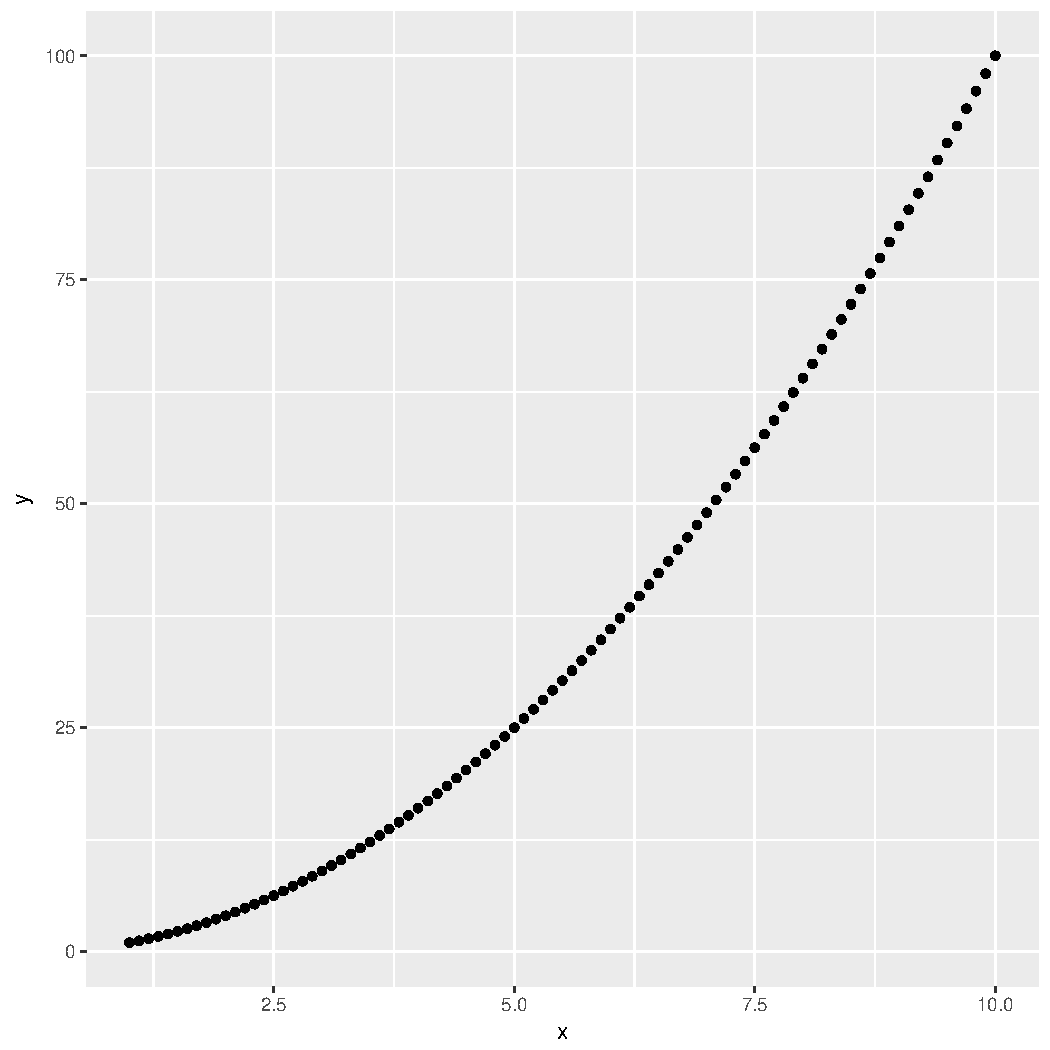
\includegraphics[width=\maxwidth]{figure/unnamed-chunk-10-1} 

\end{knitrout}



\end{document}
